\documentclass[]{amsart}

\usepackage{amssymb,amsfonts}
\usepackage[all,arc]{xy}
\usepackage{enumerate}
\usepackage{mathrsfs}
\usepackage{extarrows}
\usepackage{mathtools}
\usepackage{tikz}

\usetikzlibrary{graphs}
\usetikzlibrary{graphs.standard}
\usepackage{pifont}
\newcommand{\cmark}{\ding{51}}
\newcommand{\xmark}{\ding{55}}
\def\ZZb{\mathbb{Z}_2}
\def\ZZ{\mathbb{Z}}
\def\Soc{\rm soc}
\def\FF{\mathbb F}
\def\CC{\mathbb C}
\def\RR{\mathbb R}
\def\NN{\mathbb N}
\def\curlyB{\mathscr B}
\def\CL{\mathcal{L}}

\newcommand{\bmat}[4]{\begin{bmatrix} #1 & #2 \\ #3 & #4\end{bmatrix}}



%theoremstyle{plain} --- default
\newtheorem{thm}{Theorem}[section]
\newtheorem{cor}[thm]{Corollary}
\newtheorem{prop}[thm]{Proposition}
\newtheorem{lem}[thm]{Lemma}
\newtheorem{conj}[thm]{Conjecture}
\newtheorem{quest}[thm]{Question}

\theoremstyle{definition}
\newtheorem{defn}[thm]{Definition}
\newtheorem{defns}[thm]{Definitions}
\newtheorem{con}[thm]{Construction}
\newtheorem{exmp}[thm]{Example}
\newtheorem{exmps}[thm]{Examples}
\newtheorem{notn}[thm]{Notation}
\newtheorem{notns}[thm]{Notations}
\newtheorem{addm}[thm]{Addendum}
\newtheorem{exer}[thm]{Exercise}

\theoremstyle{remark}
\newtheorem{rem}[thm]{Remark}
\newtheorem{rems}[thm]{Remarks}
\newtheorem{warn}[thm]{Warning}
\newtheorem{sch}[thm]{Scholium}




\makeatletter
\let\c@equation\c@thm
\makeatother
\numberwithin{equation}{section}

\bibliographystyle{plain}

%--------Meta Data: Fill in your info------
\title{M3/4 P55 Algebraic combinatorics}



\date{DEADLINE AUGUST 26, 2011}

\begin{document}

\begin{abstract}
\end{abstract}

\maketitle

\tableofcontents

\section{What does the table of contents command do?}

\subsection{Check matrix}

\begin{defn}
Suppose \(A\) is a \(m \times n\) matrix over \(\ZZb\) and:
\begin{equation*}
C = \{ x \in \ZZb^n : Ax = 0\}
\end{equation*}
We call A a check matrix of the linear code $C$
\end{defn}

\begin{prop}
Suppose the check matrix $A$ of a linear code $C$ satisfies

\begin{enumerate}
	\item $A$ has no zero column
	\item $A$ has no two equal columns
\end{enumerate}
Then $C$ corrects 1 error.
\end{prop}

\begin{proof}
Suppose false. Then $d(C) \leq 2$ by proposition 1.2.
Hence by propsoition 1.5 $\exists 0\neq \in C$ s.t $wt(C) = 1 || 2$

Suppose $wt(c) = 1$. Then $c = l_i \space(=0 ... 1 ...)$ and 

$A_C = 0 \implies Al_i = 0 \ implies ith col of A = 0$ Contradiction

Suppose $wt(c) = 2$ then $c = l_i + l_j$ so 
$Ac = 0 \implies Al_u + Al_j = 0 \implies ith col of A = jth col of A$ contradiction
\end{proof}

Examples

\begin{enumerate}
\item 
\[C_3 = \{
	x \in \ZZb^6 : \begin{bmatrix}
	1 & 1 & 0 & 1 & 0 & 0 \\
	0 & 1 & 1 & 0 & 0 & 0 \\
	1 & 0 & 1 & 0 & 0 & 1
	\end{bmatrix}x = 0
\}\]
Corrects 1 error by 1.6

\item Suppose we want a code $C$ which corrects 1 error and has $3 \times n$ check matrix for some n. What is max dim of $C$?
Answer:
By 1.6 need to find largest n s.t. $\exists 3 \times n $ check matrix with distinct non zero cols (in$\ZZb^3$). Such a matrix will have as cols all non zero vectors in $\ZZb^3$ of which there a re 7, eg:

\[
A = \begin{bmatrix}
	1 & 1 & 1 & 0 & 1 & 0 & 0 \\
	1 & 1 & 0 & 1 & 0 & 1 & 0 \\
	1 & 0 & 1 & 1 & 0 & 0 & 1
	\end{bmatrix}
\]

this is a $3\times 7$ so in check matrix of code $C$ of length 7 dim 4 (by rank nullity) correcting 1 error.

This sends 16 messages abcd using codewords abcdxyz where 
\[
	x = a + b + c,\\
	y = a +b + d \\
	z = a + c + d
\]
This is called a Hamming code $\text{Ham}(3)$

\end{enumerate}
\subsection{Correcting an error}
Suppose a codeword $c$ is sent and 1 error is made, so that received vector is $c'$ which is not necessarily a code. How do we correct the error?

Well, $c' = c + l_i$ for some $i$
So

\begin{align}
	Ac' = A(c+l_i) \\
		= Ac + Al_i \\
		= Al_i \\
		= i^\text{th} \text{col of} A
\end{align}

E.g. Let $C = \text{Ham}(3)$.
Suppose received vector is $c= (1101000)^T$.

Then \[
	Ac' = \begin{pmatrix}0\\1\\0\end{pmatrix} = 6^\text{th} \text{column of }A
\]

\subsection{Hamming Codes}

\begin{defn}
Let $k\geq3$ A Hamming Code Ham$(k)$ is a code fo which the check matrix has as columns all the distinct non zero vectors in $\ZZb^k$
\end{defn}


\begin{prop}
\begin{enumerate}
	\item Ham$(k)$ has length $2^k-1$, dim $2^k-1 - k$
	\item Ham$(k)$ corrects 1 error
\end{enumerate}
\end{prop}
\begin{proof}
	\par
	\begin{enumerate}
	\item\par
		Since there are $2^k-1$ non zero vectors in $\ZZb^k$ check matrix of Ham$(k)$ is $k\times (2^k-1)$ and rank $k$
	\item\par
		Follows from 1.6 
	\end{enumerate}
\end{proof}

\begin{defn}
Let $C, C' \subseteq \ZZb^n$. Say $C$ and $C'$ are equivalent codes if there is a permutation of the coordinates sending codewords in $C$ bijectively to codewords in $C'$. (This is equivalent to permuting the columns of the checkmatrices)
\end{defn}

E.g all Hamming codes ham$(k)$ are equivalent.

We want codes that correct more than one error though. Ideally we would like to have a matrix condition that corrects lots of errors - we would like to generalize definition 1.6

\begin{prop}
Let $d \geq 2$ and let $C$ be a code wit hcheck matrix $A$. 
\begin{enumerate}
	\item\par Suppose every set of $d-1$ columns of $A$ is linearly independent. If that is true, then the minimum distance $d(C) \geq d$
	\item\par Suppose in addition to (1) that $\exists$ a set of $d$ columns of $A$ that are linerarly dependent. then $d(C) = d$
\end{enumerate}
\end{prop}

\begin{proof}
\begin{enumerate}
	\item\par Suppose false, and $d(C) \leq d-1$. Then $\exists 0 \neq c \in C$ with $wt(c) = r \leq d-1$. Write $c$ as a sum of standard basis vectors: 
	\[
		c = e_{i_1} + ... + e{i_r}
	\]

	So \[
		0 = Ac = Ae_{i_1} + ... + Ae{i_r} 
	\]
	\[
		= \text{col}i_1 + ... + \text{col}i_r
	\]

	This is a contradiction, since by the hypothesis of (1) any set of $r \leq d-1$ columns is linearly independent.

	\item\par 
	Suppose columns $i_1 ... i_d$ are linearly dependent, say

	\[
		\lambda_1 (\text{col})i_1 + ... \lambda_d(\text{col})i_d = 0, \lambda_i \in \ZZb
	\]

	As by (1) any $d-1$ columns are linearly independent, all of $\lambda_i = 1 \forall i$. Then 

	\[
		0 = \text{col}i_1 + ... \text{col}i_d
	\]

	\[
		= A(e{i_1} + ... e{i_d})
	\]

	Then $c = e{i_1} + .. + e{i_d} \in C$ and $wt(c) = d$
\end{enumerate}
\end{proof}

E.g

	Find a linear code of length 9 dimension 2 which corrects 2 errors.
	Answer:
	Check matrix $A$ should be a $7 \times 9$ matrix (of rank 7). 
	Also need code $C = \{x \in \ZZb^9: Ax = 0\}$ to have $d(C)\geq 5$ so by 1.8 want every set of 4 columns of $A$ to be linearly independent.

	Take
	\begin{equation*}
		A = \begin{bmatrix}
			\begin{matrix}
			| & | & \\
			\end{matrix}

			\begin{matrix}
			1 & \cdots & 0 \\
			  & \ddots & \\
			0 & \cdots & 1
			\end{matrix}
			\end{bmatrix}
	\end{equation*}

	Consisting of an $7 \times 7$ identity matrix and 2 columns $c_1, c_2$

	Need:
	\begin{enumerate}
		\item $wt(c_1)\geq 4, wt(c_2)\geq 4$ (otherwise $c_i$ and less than 3 columns of $I_7$ would be linearly dependent)
		\item $wt(c_1+ c_2) \geq 3$ (otherwise $c_1, c_2$ and $\leq 2$ columns of $I_7$ would be linearly dependent)	
	\end{enumerate}
	so take 

	\begin{equation*}
		A = \begin{bmatrix}
			1 & 0 \\
			1 & 0 \\
			1 & 0 \\
			1 & 1 & I_7 \\
			0 & 1 \\
			0 & 1 \\
			0 & 1 

			\end{bmatrix}
	\end{equation*}

	This defines the code
	\begin{align*}
		C &= \{ a b a a a (a +b)  b b b \qquad: \qquad a,b \in \ZZb \} \\
		  &= \{0^9, 101111000, 0100001111, 111110111\}
	\end{align*}

\subsection{Hamming bounds}

Suppose a code $C$ has length $n$ and corrects $e$ errors. How big can $|C|$ be?\\

Recall: 
\begin{align*}
	\text{for} v &\in \ZZb^n \\
		S_2(v) &= \{x \in \ZZb^n: d(x,v)\leq e\}
\end{align*}

\begin{prop}[1.9]
	$|S_e(v)| = $ sum of binomial coefficients %write this properly
\end{prop}

\begin{proof}
	Let:
	\begin{align*}
		d_i &= \text{no of: } x\in \ZZb^n \\
			&\text{s.t } d(v,x) = i
	\end{align*}
	Then:
	\[ |S_e(v)| = d_i + d_1 + ... + d+e\]
	The vectors at distance $i$ from $v$ are those vector differeing form $v$ in $i$ cooridinates of which there are: ${n \choose i}$ so $d_i = {n \choose i}$
\end{proof}

\begin{thm}[1.10, Hamming Bound]
	Let $C$ be a code of length $n$, correcting $e$ errors. \newline
	Then \[ |C| \leq \frac{2^n}{1 + n + {n \choose 2} + ... + {n \choose e}}\]
\end{thm}

\begin{proof}
	As $C$ corrects $e$ errors, the sphere $S_e(c)$ for $c \in C$ are all disjoint. Hence: \newline
	\begin{align*}
		| \bigcup_{c\in C} S_e(c)| &= |C| | S_e(c)| \\
									&= |C| (1 + n + .. + {n \choose e}) 
	\end{align*}

	Since $\bigcup_{c \in c} S_e(c) \subseteq \ZZb^n$, this gives \newline
	$|C| (1 + n + ... + {n \choose e}) \leq 2^n$
\end{proof}

Eg. Let $C$ be a linear code of length 9 correcting 2 errors. What is the maximum dimension of $C$?

Ans. By hamming bound: \newline
	$|C| \leq \frac{2^9}{1+9+{9 \choose 2}}= 2^9/46 < 2^4$
	Hense $dim(C) \leq 3$.
	We found such a $C$ of dim 2.

	is there one of dim 3?

	To find one we need a $6 \times 9$ check matrix with any 4 cols independent. \newline
	Taking \[
		A = \begin{bmatrix}
			c_1 & c_2 & c_3 \\
			| & | & | & I_6

		\end{bmatrix}
	\]

	need $c_1, c_2, c_3 \in \ZZb^6$ to satisfy: \newline

	\begin{enumerate}
		\item $wt(c_i)\geq 4 \qquad \forall i$
		\item $wt(c_i + c_j) \geq 3 \qquad \forall i\neq j$
		\item $wt(c_1 + c_2 + c+3) \geq 2$
	\end{enumerate}

	Do $\exists$ such $c_1, c_2, c_3 \in \ZZb^6$?

	Answer: No, see problem sheet 2

\subsection{Perfect Codes}
\begin{defn}
	A code $C \subseteq \ZZb^n$ is  \em{e-perfect} if $C$ corrects $e$ errors and \newline
	\[
	|C| = \frac{2^n}{1 + n + .. + {n \choose e}}
	\]

	Equivalently, the union of all the (disjoint) spheres $S_e(c)\qquad (c\in C)$ is the whole of $\ZZb^n$.
\end{defn}

1-perfect codes

\begin{prop}[1.11]
	Let $C \subseteq \ZZb^n$. Then \newline
	\[
		|C| = \frac{2^n}{1+n} \iff n=2^k-1, |C| =26 2^n-k 
	\]
	for some $k$
\end{prop}

\begin{proof}
	
	$\Rightarrow$ \newline
	If $|C| = \frac{2^n}{1+n}$ then $1 +n = 2^k$ for some $k$ \newline
	$\Leftarrow$ Clear
\end{proof}

Recall that Hamming code Ham$(k)$ has length $n= 2^k-1$, dimension $n-k$ and corrects 1 error. Hence: \newline

\begin{prop}[1.12]
	Ham$(k)$ is a 1-perfect code.
\end{prop}

Are there any \emph{e-perfect} codes for $e\geq2$

E.g.\newline
For $e=2$, we need $1+n + {n \choose 2} = 2^k$ for some integer $k$ \newline
This is quite rare, but does happen. (ask the number theory nerds)
\par
Famous theorem (van-Lint, Tietraven, 1964)

\begin{thm}
The only \emph{e-perfect} codes are:
	\begin{enumerate}
		\item $e=1$, Ham$(k)$
		\item $n=2e+1\qquad C=\{0 ... 0, 1 ... 1\}$ of dim 1
		\item $e=3, n=23, \text{dim}C = 12$, the \em{Golay code}
	\end{enumerate}

\end{thm}
Miraculous arithmetic:\newline
\[
	1 + 23 + {23 \choose 2} + {23 \choose 3} = 2^{11}
\]

%26.1.2015
Hamming bound is a result for non existence of codes $C$ of length $n$, correcting $e$ errors.

This time we will concern ourselves with an existence result


Gilbert-Varshamov bound

\begin{exmp}
Let $C$ be a linear code of length $15$, correcting $2$ errors. What is the maximum dimension of $C$?

Ans:

Hamming bound gives

\[
	|C| \leq \frac{2^15}{1+15 +{15 \choose 2}} = \frac{2^15}{|2|} < 2^9
\]
Hence $dimC \leq 8$

More on this later.
\end{exmp}

\begin{thm}[G-V bound][1.12]
Let $n,k, d$ be positive integers such that

\[
	1 + n-1 + {n-1 \choose 2} ... + {n-1 \choose d-2} < 2^{n-k}
\]

Then there exists a linear code of length $n$, dimension $k$ with $d(C) \geq d$
\end{thm}

Eg. take $n=15, d=5$

\[
	1 + 14 + {14 \choose 2} + {14 \choose 3}  = 1 + 14 + 91 + 364 < 512 = 2^9 = 2^{15-6}
\]

So G-V bound tells us that such code $C$ of dim $6$ exists.

There may or may nto exist such codes of dim 7 or 8.
Sadly neither Hamming bound or G-V bound give us anything about the answer to this.


\begin{proof}
	Assume the G-V bound equation. We want to construct a check matrix $A$ such that:\tabularnewline
	\begin{enumerate}
		\item $A$ is $(n-k) \times n$ (of rank $n-k$)
		\item any $d-1$ columns of $A$ are linearly independent
	\end{enumerate}
	We construct such a matrix inductively, column by column.

	Start by choosing the first $n-k$ columns:
	\[
		\begin{bmatrix}
		e_1 ... e_{n-k}\\
		\end{bmatrix}
	\]

	(inductive step)
	Suppose we've chosen $i$ columns $c_1, ..., c_i \in \ZZb^{n-k}$ \tabularnewline
	Where $n-k \leq i \leq n-1$ s.t any $d-1$ columns from $c_1 ... c_i$ are linearly independent. \tabularnewline
	Then:
	\[
		A_i = (c_1, ... , c_i)
	\]

	is $(n-k)*i$ and satisfies (2)

	For the inductive step we need to choose a further column $c_{i+1}$ so that $A_{i+1} = (c_1, ..., c_i, c_{i+1})$ still satisfies 2

	%But since $n-k \leq i$	we can choose a column that is not in the span of the first i columns.
	How many ``bad'' vectors are there - vectors in $\ZZb^{n-k}$ which are the sum of $\leq d-2$ fo the vectors from $c_1, ... , c_i$

	There are at most $1 + i  + {i \choose 2} + {i \choose 3} ... + {i \choose d-2}$ such vectors.

	But since $i$ is at most $n-1$, this is less than $2^n-k$ by the G-V bound. So therefore there is a vector in $\ZZb^{n-k}$ that is not a sum of $\leq d-2$ of the vectors $c_1, ..., c_i$. Hence the matrix

	\[
		A_{i+1} = (c_1, ..., c_i, c_{i+1})
	\]
	satisfies property (2)

	By this inductive step we construct $A_i$ for $i = n-k, ..., n$. The matrix $A = A_n$ is the required check matrix.	
\end{proof}

\subsection{The Golay Code}
This is a 3-perfect code of length $23$, dimension $12$

To construct it we first construct the \emph{extended} Golay code $G_24$
Start with $H = Ham(3)$, check matrix:

\[
	\begin{bmatrix}
	1 & 1 & 1 & 0 & 1 & 0 & 0  \\
	1 & 1 & 0 & 1 & 0 & 1 & 0  \\
	1 & 0 & 1 & 1 & 0 & 0 & 1
	\end{bmatrix}
\]

And its reverse K, with check matrix

\[
	\begin{bmatrix}
	0 & 0 & 1 & 0 & 1 & 1 & 1\\
	0 & 1 & 0 & 1 & 0 & 1 & 1\\
	1 & 0 & 0 & 1 & 1 & 0 & 1
	\end{bmatrix}
\]

Add a parity check bit (= sum of bits) to $H, K$ to get length 8 codes $H', K'$
% list hamming H' and K' codewords here


Note.1 $H', K'$ are linear codes of length 8 dim 4.
Note.2 All codewords are have weight 0, 8 or 4.

Taking the 14 codewords of weight 4 in $H'$ you'll see that you can define a collection of blocks, forming a 3-design. ($v=8$ points, $k=4$ (size of block))

\begin{prop}[1.13]
$H \cap K = \{0^7, 1^7\} \qquad \&  \qquad H'\cap K' = \{0^8, 1^8 \}$
\end{prop}

\begin{proof}
Let $v\in H\cap K$

\begin{align*}
	H &= \begin{pmatrix}
		1 & 1 & 1 & 0 & 1 & 0 & 0 \\
		1 & 1 & 0 & 1 & 0 & 1 & 0 \\
		1 & 0 & 1 & 1 & 0 & 0 & 1 \\
	\end{pmatrix} \\
	v \in H & \qquad \Rightarrow \qquad v = abcd, a+b+c, a+b+d, a+c+d\\
\end{align*}
\begin{align*}
\text{So} \qquad v \in K \quad\Rightarrow\quad \\
	c + (a+b+c) + (a+b+d) + (a+c+d) = 0 &\quad\rightarrow\quad a +c = 0\\
	b + d + (a + b + d) + (a + c +d)= 0 &\quad\rightarrow\quad c + d = 0 \Rightarrow a = b = c = d \\
	a + d + (a + b + c) + (a + c +d)= 0 &\quad\rightarrow\quad a + b = 0 \Rightarrow v = 0^7\quad\text{or}\quad 1^7
\end{align*}
\end{proof}

\subsection{Solutions to sheet 1}
\begin{proof}[3a]
	$C = \{v \in \ZZb^n : wt(v) \text{even} \}$
	Check matrix $(1\; 1\;...\; 1)$
	\begin{align*}
		\text{Then}\quad	 C &= \{v \in \ZZb^n : (1\;1\;...\;1)v = 0\}\\
					  &= (v_1\;...\;v_m)^T
	\end{align*}
\end{proof}

\begin{proof}[7]\hfill\newline
	$T(n):$ vertices = paris from $\{1\;...\;n\}$\newline
	join $A, B$ if $A\cap N \neq \emptyset$\newline
	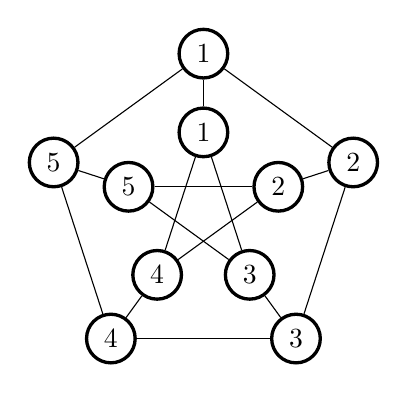
\begin{tikzpicture}[every node/.style={draw,circle,very thick}]
	  \graph[clockwise, radius=2cm] {subgraph C_n [n=5,name=A]};
	  \graph[clockwise, radius=1cm] {subgraph I_n [n=5,name=B]};

	  \foreach \i in {1,2,3,4,5}{\draw (A \i) -- (B \i);}
	  \newcounter{j}
	  \foreach \i in {1,2,3,4,5}{%
	  \pgfmathsetcounter{j}{ifthenelse(mod(\i+2,5),mod(\i+2,5),5)}
	  \draw (B \i) -- (B \thej);
	  }
	  %fix labels here (12) 34 15 23 45 // 35 25 24 14 13

	\end{tikzpicture}
	$T(n)$ is strongly regular.
	\begin{enumerate}
		\item \par
			$ij$ joined to all pairs in $\{1,\;...,\;n\}\setminus ij $\newline
			regular of valency = ${n-2 \choose 2}$
		\item \par
			no. of common neighbours of $ij $ 2-joined vertices $, kl = {n-4 \choose 2}$
			%draw pic
		\item \par no. of common neighborus of 2 non-joined veritces is ${n-3 \choose 2}$
			%draw pic
	\end{enumerate}
\end{proof}
\begin{proof}[6]
	Steiner triple sistem is a 2-design with $k=3$, any 2 points in one block. \newline
	Set $X$ of $v$ points. Collection $B$ of blocks of size $3$. Any point is in $v$ blocks. Any 2 points in one block.\\
	a)\hfill \\
		$X = \ZZb^n \setminus 0$ \\
		Blocks $=$ subsets $\{x,y, x+y\} \qquad (x\neq y \in x)$ \\
		This is a STS:
			\begin{enumerate}
				\item \hfill \\
				Let, $x,y$ be 2 pioints. The lie in the block $\{x,y x+y\}$\\
				If the lie in a block $\{v,w, v+w\}$ then:\\
				\[
				x,y = \begin{matrix}
						v, w \\
						v, v+w \\
						w, v+w \\
					  \end{matrix}
				\]
				and in each case $\{v,w, v+w\} = \{x,y x+y\} $ so $x,y$ lie in exactly 1 block. Note $|X| = 2^n -1 $
				\item \hfill \\
				Let $x \in X$. The no of blocks containing $x\qquad \{x,y, x+y\}$.\\ 
				This no is $\frac{2^n-2}{2} = 2^{n-1}-1 = r$
			\end{enumerate}
	b)\hfill \\
	STS, $|X| = v$. Count pairs $(xy, B)$ with $x,y \in B$.\\
	\begin{align*}
		\text{No. of pairs} \quad &= \quad (\text{no of choices xy})\times 1 \\
								  &= {v \choose 2}\\
	\end{align*}

	\begin{align}[rabbit]
	\text{this no is}\\
	(\text{No. of B's}) \times {3 \ choose 2} = 3b \\
	\text{So:}\quad {v \choose 2} = 3b \Rightarrow v(v-1) = 6b\\
	\end{align}
	Hence $b | v(v-1)$ Also 
	\begin{align*}
		b= \frac{vr}{k} = \frac{vr}{3} \Rightarrow \frac{v(v-1)}{6} = \frac{vr}{3}\Rightarrow r = \frac{v-1}{2}
	\end{align*}
	So $v$ is odd\\
	c)\hfill \\
	Let $v\leq 12. 6| v(v-1)$ and $v$ odd.
	Then $v = 3, 7 \;\text{or}\; 9$\\
	$v = 3$: Trivial STS.\\
	$v = 7$: There is one by previous part $\ZZb^3\setminus 0$ STS.\\
	$v = 9$: Yes. \hfill \\
	Points $\{0,\;1,\;...\;\}8$. \\
	Let: 
	\begin{align*}
	A = \begin{pmatrix}
			0 & 3 & 6 \\
			1 & 4 & 7 \\
			2 & 5 & 8 \\
		\end{pmatrix}
	\end{align*}
	Take as blocks of size 3:
	\begin{description}
		\item[Rows of ATu]
		$036, \quad 147,\quad 256$
		\item[Cols of ATu]
		$012, \quad 345, \quad 678$
		\item[Triples with 1 pt from each row and column of $A$Tu]
		$048, \quad 057, \quad 138, \quad 156, \quad 237, \quad 246$\\
	\end{description}
	Let $x,y$ be points. If $x,y$ are in the same row or col they are in a unique block. If not $x,y$ in a unique block of type 3.
\end{proof}


%Guest lecture John Britnell
\begin{align*}
	H = Ham(3) \qquad & \qquad H' = H + \ \text{parity check}\\
	K = \text{reverse of}\; H \qquad & \qquad K' = K + \ \text{parity check}
\end{align*}

\begin{defn}[The exteded Golay Code $G_24$]\hfill\\
$G_24$ consists of all vectors in $\ZZb^24$ of the form:
\begin{align*}
(a +x, b +x, a + b + x), \qquad&\qquad \text{where} a,b\;\in H\\
(\xlongleftrightarrow{8}, \xlongleftrightarrow{8}, \xlongleftrightarrow{8}), \qquad&\qquad \text{and}\;x\in L\\
\end{align*}

\begin{enumerate}
	\item\hfill\\
	$0^24\qquad \qquad a = b = x = 0^8$
	\item\hfill\\
	$1^24\qquad \qquad a = b = 0^8 \qquad x = 1^8$
	\item\hfill\\
	$(0^8, 1^8, 0^8) a =x = 1^8 \qquad b=0^8$
	\item\hfill\\
	$(0^8, 0^8, 0^8) a = b =x = 1^8$
	\item\hfill\\
	$a = 10001110, b = 10011001, x = 01001011$
\end{enumerate}
\end{defn}

\begin{prop}
$G_24$ is a linear code of dimension 12.
\end{prop}
\begin{proof}
	\begin{enumerate}
		\item[Linear]\hfill\\
			$0^24 \in G_24$

		\item[Closure]\hfill\\
			Suppose $a_1, a_2, b_1, b_2 \in H\, \qquad x_1, x_2 \in K'$\\
			Then 
			\begin{align*}
				&(a_1 + x_1, b_1 + x_1, a_1 + b_1 + x_1) + (a_2 + x_2, b_2 + x_2, a_2 + b_2 + x_2) =\\
					&= (a_1 + a_2 + x_1 + x_2, b_1 + b_2 + x_1, + x_2, a_1 + a_2 + b_1 + b_2+ x_1 + x_2) \in G_24\\
					&\text{Since:} \qquad a_1, a_2, b_1, b_2 \in H\, \qquad x_1, x_2 \in K'
			\end{align*}
		\item[Dimension]\hfill\\
		Suppose: $a_1 + x_1, b_1 + x_1, a_1 + b_1 + x_1) = (a_2 + x_2, b_2 + x_2, a_2 + b_2 + x_2)$\\
		Then:\\
		\begin{align*}
			a_1 + x_1 &= a_2 + x_2\\
			b_1 + x_1 &= b_2 + x_2\\
			a_1 + b_1 + x_1 &= a_2 + b_2 + x_2\\
		\end{align*}
			Adding $x_1 = x_2$, we get $a-1 = a2$ and $b_1 = b_2$\\
			So distinct choices of $(a,b,x)$ give distinct elements of $G_24$.\\
			\begin{align*}
				\text{So:} \quad |G_24| &= \text{number of triples}\qquad (a,b,x) \qquad \qquad a,b \in H' \quad x\in K'\\
				&= |H'|^2  |K'| = 2^4 \times 2^4 \times 2^4 = 2^12
			\end{align*}
			So $dim G_24 = 12$\\
		\item[Basis]\hfill \\
			Note that $(a+x, b+x, a+b+x) = (a,0,a) + (0,b,b) + (x,x,x)$ (all of these in $G_24$\\
			So if $a_i, b_i, x_i \quad (1\leq i \leq 4)$ are bases for $H', H', K'$ respectively, then:\\
			$(a,0,a) , (0,b,b) , (x,x,x) \qquad (1\leq i \leq 4)$ is a basis for $G_24$
	\end{enumerate}
\end{proof}
\begin{thm}
	$G_24$ has minimum distance 8\\
\end{thm}[1.15]
\begin{proof}
	Needs multiple steps. \\
	For $v,w \in \ZZb^n$ define $[v,w] = \text{number of places where $v$ and $w$ are both 1}$\\
\end{proof}
\begin{prop}[1.16]\hfill\\
	Let $v,w \in \ZZb^n$\\
	\begin{enumerate}
		\item $wt(w) = wt(v) + wt(w) = 2[v,w]$\\
		\item If 4 divides $wt(w)$ and $wt(w)$ then 4 divides $wt(v+w)$ iff $[v,w]$ is even\\
	\end{enumerate}
\end{prop}
\begin{proof}
	Let $r = wt(v),\quad s = wt(w),\quad t = [v,w]$\\
	Reordering coordinates as necessary, we can write:\\
	\[
		\begin{matrix}
			& \xlongleftrightarrow{t} & \xlongleftrightarrow{r-t} & \xlongleftrightarrow{s-t}\\
		v  =& 1 ... 1  				  &1 ... 1 					  &0 ...0		    & 0 ... \\
		w  =& 1 ... 1  				  &0 ... 0 					  &1 ...1		    & 0 ... \\
		w+w=& 0 ... 0  				  &1 ... 1 					  &1 ...1		    & 0 ... \\
		\end{matrix}
	\]
	Therefore let $wt(v+w) = (r-t) + (s-t) = r +s - 2t$\\
	2) follows immediately from 1.
\end{proof}

\begin{prop}\hfill\\
	If $a,b,x \in \ZZb^n$ then $[a,x] + [b,x] + [a+b,x]$ is even.\\
\end{prop}
\begin{proof}
	Let $r = [a,x],\qquad s = [b,x]$ and let $n$ be the number of places where $a,b,x$ all have 1.\\
	Reordering coordinates we can write
		\[
			\begin{matrix}
				& \xlongleftrightarrow{n} & \xlongleftrightarrow{r-n} & \xlongleftrightarrow{s-n}\\
			x  =& 1 ... 1  				  &1 ... 1 					  &1 ...1			&1 ...1		    & 0 ...  \\
			a  =& 1 ... 1  				  &1 ... 1 					  &0 ...0			&1 ...1		    & *  \\
			b  =& 1 ... 1  				  &0 ... 0 					  &1 ...1			&1 ...1		    & *  \\
			a+b=& 0 ... 0  				  &1 ... 1 					  &1 ...1			&0 ...0		    & *  \\
			\end{matrix}
		\]
		We have $[a+b, x] = (r-n) + (s-n) = (r+s-2n)$\\
		So: $[a,x] + [b,x] + [a+b,x] = r+s + (r+s-2n) = 2(r+s-n)$ which is even
\end{proof}

\begin{prop}[1.18]\hfill
If $c \in G_24$ then 4 divides $wt(c)$.
\end{prop}

\begin{proof}\hfill\\
	We have $c = (a+x, b+x, a+b+x)\qquad a,b \ in H', x\in K'$\\
	So: 
	\[c \underset{v}{(a,b, a+b)} \underset{+}{+} \underset{w}{(x,x,x)}\]
	Since $a,b \in H'$ and $x\in K'$ we know 5 divides $wt(a), wt(b), wt(x)$.
	So 4 divides $wt(v), wt(w)$\\
	And $[v,w] = [a,x] + [b,x] + [a+b, x]$ which is even (prop 1.17)\\
	So $wt(v+w)$ is divisible by 4 by proposition 1.16 (2)\end{proof}



\end{document}

